\documentclass{ludis}

% xelatex
\usepackage{fontspec}
\usepackage{xunicode}
\usepackage{xltxtra}

% languages
\usepackage{fixlatvian}
\usepackage{polyglossia}
\setdefaultlanguage{latvian}
\setotherlanguages{english,russian}

% graphics
\usepackage{pgfplots}
\usepackage{graphicx}
\DeclareGraphicsExtensions{.png,.eps}

% fonts
\setmainfont[Mapping=tex-text]{DejaVu Serif}
\setsansfont[Mapping=tex-text]{DejaVu Sans}
\newfontfamily\russianfont{DejaVu Serif}

% toc
\setcounter{secnumdepth}{3}
\setcounter{tocdepth}{3}

% formatting
\usepackage{footnote}

% bibtex
\usepackage[pdfauthor={Emīls Šolmanis},%
pdftitle={Tehnoloģiju izvēle mašīnmācīšanās eksperimentu veikšanai},%
pdfkeywords={machine learning, choice of technology, software engineering},%
hidelinks=true,%
pagebackref=false,%
xetex]{hyperref}
\hypersetup{colorlinks=false}
\urlstyle{same}
\usepackage{cite}


%% \usepackage{amsmath}
%% \usepackage{amssymb}
%% \usepackage{enumerate}

\fakultate{Datorikas}
\nosaukums{Tehnoloģiju izvēle mašīnmācīšanās eksperimentu veikšanai}
\darbaveids{Kursa}
\autors{Emīls Šolmanis}
\studapl{es09260}
\vaditajs{Asoc. prof., Dr. dat. Jānis Zuters}
\vieta{Rīga}
\gads{2012}

\begin{document}
\maketitle

\begin{abstract-lv}
  Darba mērķis ir izpētīt tehnoloģijas, kas varētu tikt lietotas dažādu mašīnmācīšanās eksperimentu implementācijā. Mērķis ir katram no eksperimentiem atrast optimālu risinājumu implementācijai -- programmēšanas valodas, pieejamo ietvaru, bibliotēku un algoritmu ziņā, ņemot vērā veiktspēju, prognozēto darbietilpību un galaprodukta uzturamību.
  \keywords{mašīnmācīšanās, tehnoloģiju izvēle, programminženierija}
\end{abstract-lv}

\begin{abstract-en}
  The aim of this thesis is to explore the available options that could be used in the implementation of several machine learning experiments. For each of these experiments, the goal is to find the optimal means of implementation in terms of programming language, available frameworks, libraries and algorithms, considering the performance, estimated development effort and maintainability of the final product.
\keywords{machine learning, choice of technology, software engineering}
\end{abstract-en}

\tableofcontents

\specnodala{Ievads}
Darbā apskatītas un salīdzinātas mūsdienās pieejamās tehnoloģijas mašīnmācīšanās eksperimentu implementēšanai. Hipotēze -- dažas no tām ir labākas un vairāk piemērotas šim mērķim par citām.

Tehnoloģiju salīdzināšanai noteikti gan konkrēti, empīriski izmērāmi kritēriji, piemēram, veiktspēja un prognozētā darbietilpība, taču ņemti vērā arī nozīmīgākie subjektīvie apsvērumi -- piemēram, cik liels ir nepieciešamais sākotnējais darba ieguldījums tehnoloģijā (uzstādīšana, konfigurēšana u. tml.), pieejamā dokumentācija un tās kvalitāte.

Tiek pieņemts, ka visām izvēlētajām tehnoloģijām jābūt maksimāli platform-neatkarīgām. Šajā gadījumā, noteiktais ierobežojums ir spēja apskatāmo objektu uzstādīt un darbināt ar x86 arhitektūras procesoriem uz Linux (kodola versija 2.4 un jaunāka), Mac OS X (Snow Leopard un jaunāka) un Windows (versija 7 un jaunāka).

Darbā apskatītie tehnoloģiju aspekti ir programmēšanas valoda, pseido-gadījumskaitļu ģenerēšana, lineārā algebra un paralēlās programmēšanas iespējas.

Apskatāmās problēmas izmērs neļauj apskatīt visas iespējamās alternatīvas, tādēļ problēmas risināšanas gaitā tiks apskatītas tikai populārākās un / vai nozīmīgākās iespējas. Tā kā ir hipotēze, ka kāda no tehnoloģijām ir labāka par citām, ir nepieciešami kritēriji, pēc kā tehnoloģiju vērtēt. Problēmas risināšanas gaitā, dažādām tehnoloģijām tika eksperimentāli noteikta veiktspēja un aptuveni izvērtēta prognozētā darbietilpība.

Darba rezultāti parāda, ka hipotēze ir pareiza. Eksistē tehnoloģijas, kas ir vairāk piemērotas mašīnmācīšanās eksperimentiem, nekā citas. Rezultāti pierāda, ka mūsdienu apstākļos vislabāk ir izvēlēties kādu no brīvi tipizētajām, dinamiskajām valodām, kurām vajadzības gadījumā ir iespēja izsaukt gatavas zemāka līmeņa bibliotēku funkcijas (piemēram, kādu BLAS pakotni).

\chapter{Uzdevuma izpēte}
\section{Problēmas būtība}
Mūsdienās ir pieejams plašs tehnoloģiju klāsts, pirms vispār ķerties pie kāda konkrēta uzdevuma risināšanas ir jāizvēlas veids, kādā to darīt. Parasti ir jāizdara izvēle starp dažādām prorammēšanas paradigmām, tad konkrētām valodām, dažādiem algoritmiem, bibliotēkām un ietvariem, ko izmantot. Gandrīz nekad nav viena risinājuma, kas būtu labs visos aspektos un ir jāpieņem dažādi kompromisi -- piemēram, produkta izstrādes sākumā, prototipēsanas stadijā, bieži vien ir svarīgāk iespējami ātri izveidot strādājošu prototipu, nepievēršot pastiprinātu uzmanību ātrdarbībai.

Ir hipotēze, ka, izvēloties pietiekami specifisku problēmu, ne visi ieguvumi un zaudējumi ir vienlīdzīgi, tādēļ ir iespējams atrast kādu tehnoloģiju konfigurāciju, kas ir labāka par citām, kuras izmantošanas ieguvumi būtu ievērojami lielāki par zaudējumiem.

Pieņemts, ka mašīnmācīšanās ir mākslīgā intelekta izpētes apakšnozare, kas izstrādā algoritmus un metodes, kas balstoties uz empīriskiem datiem un novērojumiem ļauj datoram izveidot kādu uzvedības modeli.

Darbā tiek pieņemts, ka uzdevuma implementācijas gaitā jārisina šādi tipiski mašīnmācīšanās eksperimentu aspekti:
\begin{itemize}
\item pseido-gadījumskaitļu ģenerēšana;
\item lineārā algebra, uzsvars uz matricu / vektoru aritmētiku;
\item paralēlā programmēšana;
\end{itemize}

Šajā darbā tiek apskatīta izvēle starp:
\begin{itemize}
\item programmēšanas paradigmām;
\item programmēšanas valodām;
\item vienas problēmas dažādiem risināšanas algoritmiem un / vai pieejām;
\end{itemize}

\section{Programmēšanas paradigmas} \label{sec:paradigms}
Ir trīs populāras programmēšanas paradigmas, ko saista ar mākslīgā intelekta un mašīnmācīšanās izpēti un eksperimentiem -- deklaratīvā, funkcionālā un imperatīvā / procedurālā. 

Var teikt, ka funkcionālā programmēšana radās tieši mākslīgā intelekta izpētes dēļ, jo īpaši valoda Lisp, un ar šo nozari tiek saistīta jau praktiski kopš tās pirmsākumiem ~\cite{hist_lisp}. 

Līdzīgi ir ar deklaratīvo programmēšanu. Tā gan radās mazliet vēlāk, bet arī šīs paradigmas viens no senākajiem un populārākajiem pārstāvjiem, Prolog, jau no pirmsākumiem tiek saistīts ar mākslīgā intelekta izpēti, taču ne tik izteikti kā Lisp.

Imperatīvās paradigmas nozīme mašīnmācīšanās un mākslīgā intelekta izpētes jomā pieauga gandrīz vienlaicīgi ar Lisp popularitātes kritumu, un šiem notikumiem bija vienots cēlonis -- personālo datoru cenas kritums, kas ļāva izpildīt jebkādas programmas uz jebkura datora. 

Jāpiebilst, ka lai arī šī paradigma sākotnēji nespēlēja nopietnu lomu tieši mašīnmācīšanās izpētē, tās viens no pirmajiem pārstāvjiem, FORTRAN, ļāva ļoti efektīvi implementēt atsevišķas, svarīgas tehnoloģiju daļas, piemēram, matricu aritmētiku. Līdzīgas iespējas bija arī jaunākām valodām, C un C++. Tas stipri ietekmēja šīs paradigmas izaugsmi un popularitāti brīdī, kad skaitļošanas resursi kļuva lētāki un pieejamāki.

Mūsdienās vērojams stabils dinamisko, multi-paradigmu valodu lietošanas pieaugums un tradicionālo funcktionālo valodu popularitātes kritums ~\cite{tiobe_index}. Tādējādi pamazām robeža starp paradigmām izplūst, un vairs nav retums pat viena projekta ietvaros sastapties ar vairākām paradigmām. Pat C++ jaunajā standartā ir spēris soli tuvāk funkcionālajai programmēšanai ieviešot {\em lambda}-izteiksmes ~\cite{iso_cpp11}.

\section{Programmēšanas valodas} \label{sec:languages}
Kā minēts sadaļā ``\nameref{sec:paradigms}'' ar mākslīgā intelekta un mašīnmācīšanās izpēti ir saistītas, galvenokārt, deklaratīvā, funkcionālā un imperatīvā paradigma. No funkcionālās un deklaratīvās paradigmas tās gan ir vairāk konkrētas valodas, nekā visa paradigma.

\subsection{Lisp}
Lisp vēsturiskie pirmsākumi meklējami tieši mākslīgā intelekta izpētes jomā ~\cite{hist_lisp}. Tika pat būvēti speciāli, Lisp izpildei optimizēti, datori. Taču ap 1990. gadu Sun, IBM un Apple ražotu personīgo datoru cenas sāka kristies un to veiktspēja strauji augt. Drīz tie varēja izpildīt Lisp programmas ātrāk par specializētajiem Lisp datoriem un to ražošana tika pārtraukta ~\cite[p.~209--210]{crevier_1993}. Tas manāmi samazināja arī Lisp popularitāti un lietojumu visā pasaulē, t. sk. mākslīgā intelekta izpētē.

Lisp valodai ir vairākas īpatnības, kas to padara pievilcīgu mākslīgā intelekta izpētei -- piemēram, šajā valodā programmas teksts sastāv no saraksta datu struktūrām un ir tieši tādi paši ievaddati, kā jebkas cits. Tas ļauj viegli rakstīt pašmodificējošas programmas un dažādas citas dinamiskas sistēmas. Minētie apstākļi un valodas piederība funkcionālajai paradigmai padara to par labu izvēli dažādu ``domājošu'' un adaptīvu sistēmu izveidei, taču šis pats apstāklis to padara neērti lietojamu matricu algebrai un intensīvām skaitļošanas operācijām, ja to dara bez speciālām optimizācijām.

Apskatot tieši mašīnmācīšanās nozari, Lisp biežāk tiek lietots valodas apstrādē (semantiskā analīze) un grafu apstrādē (piemēram, Beijesa tīkli), bet ne tik daudz ar intensīvu skaitļošanu saistītiem eksperimentiem, piemēram, neironu tīkliem.

Par spīti valodas un paradigmas popularitātes kritumam pēc Lisp specializēto datoru ražošanas pārtraukšanas, pēdējos gados tas ir stipri atguvis popularitāti, taču ne tā tradicionālajā Common Lisp implementācijā un formā.

Funkcionālās programmēšanas pēdējā laika augošajai popularitātei pamatā ir divas konkrētas valodas -- Scala un Clojure. Tās abas ir balstītas uz JVM. Tas ļauj tām abām lietot gandrīz visas pastāvošās Java bibliotēkas un ietvarus, tādējādi var lietot funkcionālo programmēšanu un, ja rodas tāda nepieciešamība, izmantot esošu Java bibliotēku vai rakstīt tādu no jauna un integrēt ar sākotnējo valodu.

Scala ir 2004. gadā izlaista multi-paradigmu valoda. Tā ir objekt-orientēta un stingri tipizēta, taču ar uzsvaru uz paralēlismu un spēcīgu funkcionālās programmēšanas atbalstu ~\cite{scala_org}.

Otra valoda, Clojure, ir 2007. gadā izveidota Lisp implementācija. Arī tā tika veidota ar stingru uzsvaru uz paralēlismu, taču tā ir Lisp implementācija, līdz ar to nav stingri tipizēta, visas tās programmas ir ievaddati un tā nav objekt-orientēta ~\cite{clojure_org}.

\subsection{Prolog}
Prolog ir viena no pirmajām deklaratīvajām formālajā loģikā balstītajām valodām. Tās sākotnējais mērķis bija valodas apstrāde. Arī tai, līdzīgi kā Lisp, bija mēģinājumi konstruēt specializētus datorus, taču masu ražošanu tie tā arī nesasniedza.

Nopietnu popularitāti valoda tā arī nekad nav sasniegusi. Tā kā tā ir deklaratīva, t.i., tās izpilde balstās uz deklarētiem predikātiem un faktiem, parasti programmas tajā ir par lēnu, lai būtu piemērojamas reāliem eksperimentu scenārijiem ar lieliem datu apjomiem.

\subsection{Imperatīvās valodas}
 Kaut arī šī paradigma ir tikpat veca kā funkcionālā vai deklaratīvā, imperatīvās un procedurālās valodas tieši ar mašīnmācīšanos tiek saistītas salīdzinoši nesen. Galvenais to popularitātes pieaugums sākās līdz ar Lisp norietu un personīgo datoru izmaksu kritumu ap 1990. gadu. Liels šī popularitātes pieauguma iemesls bija pārāka veiktspēja. Tādas valodas, kā FORTRAN, C, C++, ir salīdzinoši viegli pārtulkot mašīninstrkcijās mūsdienu arhitektūrām, un tādēļ parasti tās strādā ievērojami ātrāk par funkcionālajām alternatīvām. Tas ļāva eksperimentēt ar lielākiem datu apjomiem un ātrāk izmēģināt tehnikas, kuras balstījās uz intensīvu skaitļošanu.

Mūsdienās mašīnmācīšanās nozarē imperatīvā programmēšana tiek plaši lietota, bet runājot par imperatīvajām valodām, sīkāk jāizdala divi to paveidi -- vecākās tradicionālās un jaunās, multi-paradigmu.

\subsubsection{Tradicionālās imperatīvās valodas}
Par tradicionālām var saukt tās imperatīvās programmēšanas valodas, kuras atbalsta tikai imperatīvo pieeju. Tipiskākie un nozīmīgākie pārstāvji ir FORTRAN, C un C++. Lietošanas iemesli mašīnmācīšanās nozarē ir tie paši, kas vēsturiski -- ātrdarbība. Ja nepieciešams maksimāli izmantot ierobežotos datora resursus, iespējams pat rakstīt programmas fragmentus mašīnkodā, šajās valodās to parasti ir iespējams viegli izdarīt. Taču līdz ar lielāko kontroli parasti palielinās arī izstrādes laiks un sarežģītība.

\subsubsection{Multi-paradigmu valodas}  \label{sec:multi_paradigm}
Šī ir salīdzinoši jauna pieeja, un tai ir strauji augošs piekritēju skaits visās nozarēs, ne tikai zinātnē. Lai arī pirmie pārstāvji parādījās salīdzinoši sen, līdz pat nesenam laikam datoru skaitļošanas jauda nebija gana liela, lai šīm valodām būtu praktisks pielietojums. Šīs valodas neuzspiež programmētājam kādu konkrētu pieeju un ļauj ērti strādāt vairākās, parasti vismaz imperatīvajā un funkcionālajā. Tas, savukārt, parasti samazina nepieciešamo izstrādes laiku. Tipiskie pārstāvji ir Python, Ruby, Scala.

\section{Algoritmu izvēle}
Šī problēmas daļa ir saistīta ar to, ka pat ja ir izvēlēta kāda konkrēta implementācijas valoda, atsevišķas problēmas daļas var risināt ar dažādiem algoritmiem, starp kuriem nav strikti nosakāms ``labākais'', jo ir vairāki cits citu ietekmējoši izvēles kritēriji un nepieciešams rast kompromisu. 

Tipisks piemērs ir gadījumskaitļu ģeneratori. Ir daudz dažādu algoritmu, kas paredzēti pseido-gadījumskaitļu ģenerēšanai. Tos visus var inicializēt ar sistēmas gadījumskaitļu ģeneratoru, piemēram, \texttt{/dev/random} Linux sistēmās, jo sistēmas gadījumskaitļu ģeneratori ir parasti tiek uzskatīti par kriptogrāfiski drošiem gadījumskaitļu ģeneratoriem. Taču tie nevar ģenerēt pietiekoši garas gadījumskaitļu virknes pietiekoši ātri, tiem ātri sāk trūkt entropijas un nākas lietot pseido-gadījumskaitļu ģeneratorus ~\cite{man_random}.

Taču izvēloties pseido-gadījumskaitļu ģenerēšanas algoritmu ir jāņem vērā vairāki parametri:
\begin{itemize}
\item gadījumskaitļu virknes perioda garums;
\item algoritma ātrdarbība;
\item gadījumskaitļu varbūtības sadalījums -- ne visiem algoritmiem tā ir vienmērīga.
\end{itemize}

\section{Ietvaru, bibliotēku un implementāciju izvēle}
Katram konkrētam algoritmam ir iespējami vairāki implementācijas veidi. Mūsdienās bieži vien izmantotajai bibliotēkai vairs pat nav jābūt rakstītai tajā pašā valodā, kādā rakstīts projekts, kurā tā tiek izmantota. Piemēram, saišu redaktors var savienot C++ kodu ar kompilētu FORTRAN bibliotēku. No Python valodas var izsaukt C bibliotēkas. Scala un Clojure var lietot gandrīz jebko, kas ir palaižams uz JVM, t.i., arī Java bibliotēkas. Mūsdienās šīm starpvalodu robežām ir tieksme kļūt arvien plānākām.

Ņemot vērā šos apstākļus, rodas plašas izvēles iespējas arī tad, ja ir izvēlēts optimāls algoritms. Labs piemērs ir lineārās algebras implementācijas -- tradicionālās BLAS / LAPACK bibliotēkas ir implementētas FORTRAN. Taču dažādu iemeslu -- piemēram, vieglāk saprotamākas programmētāja saskarnes dēļ, bieži ir vērts apsvērt augstāka līmeņa implementācijas, īpaši tad, ja veiktspēja nesamazinās. Var arī atmest BLAS / LAPACK un meklēt pilnīgi jaunas lineārās algebras darbību implementācijas.

\chapter{Risinājums}
\section{Paradigmas izvēle} \label{sec:paradigm_choice}
Pašās paradigmās nav ierobežojumu, kas principiāli liegtu izmantot kādu konkrētu paradigmu mašīnmācīšanās eksperimentiem. Taču kā aprakstīts sadaļā ``\nameref{sec:languages}'', deklaratīvā paradigma un Prolog nav derīga praktiskiem mašīnmācīšanās eksperimentiem, ja datu apjoms ir liels. Tādējādi, izvēle ir starp funkcionālo un imperatīvo.

Katrai ir savas priekšrocības. Funkcionālās paradigmas pieeja izvairās no programmas stāvokļa uzglabāšanas un maināmiem objektiem, kas ievērojami atvieglo atkļūdošanu, testēšanu un padara to vieglāk paralelizējamu. Tradicionālo imperatīvo valodu galvenā priekšrocība parasti ir to ātrdarbība, bet arī iespēja glabāt stāvokli reizēm ir nepieciešama un ir labi, ja to nav jāemulē.

Kā redzams, neviena pieeja nav perfekta, katrai ir savi trūkumi. Tādēļ var lietot multi-paradigmu valodas un izmantot labāko no abām. To lielākais trūkums -- tā kā tās parasti ir vāji tipizētas un, vismaz kādā līmenī, interpretējamas, tās parasti ir arī vismaz mazliet lēnākas par tradicionālajām imperatīvajām. 

Praktiskie eksperimenti \ref{fig:bench_game} ~\cite{bench_game} rāda, ka kopējās veiktspējas atšķirības nav ļoti nozīmīgas un tās nebūtu jāpieņem par izšķirošo faktoru mašīnmācīšanās eksperimentu izstrādē. Ir redzama tendence, ka imperatīvās ir ātrākas par funkcionālajām un funkcionālās ir ātrākas par multi-paradigmu, taču pat lēnākās valodas ir pietiekami ātras praktiskiem eksperimentiem. Jo īpaši tādēļ, ka parasti no augstāka līmeņa valodām ir iespējams izsaukt zemāka līmeņa implementācijas. Tādējādi var, piemēram, rakstīt programmas loģiku vai grafisko saskarni Python, bet matricu algebru tik un tā rēķināt ar kādu C vai FORTRAN rakstītu BLAS implementāciju.
\begin{figure}
  \centering
  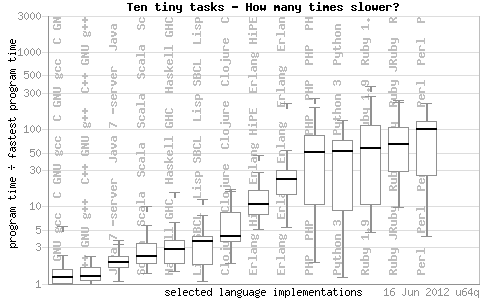
\includegraphics{img/bench_game}
  \caption{Valodu veiktspējas salīdzinājums}
  \label{fig:bench_game}
\end{figure}

\section{Valodas izvēle}
Kā tika parādīts sadaļā ``\nameref{sec:paradigm_choice}'', paradigmai nav fundamentālas nozīmes un galvenie optimizācijas parametri šajā jomā ir pieejamās iespējas un prognozējamā darbietilpība. Tā kā katram konkrētam eksperimentam funkcijpunktu skaits, riski un citi faktori ir konstanti, vienīgais mainīgais ir koda rindiņu skaits viena funkcijpunkta izpildei.

Kā redzams grafikā, koda rindiņu skaitam funkcijpunkta izpildei ir dilstoša tendence pārejot no tradicionālajām imperatīvajām valodām (C, FORTRAN) uz funkcionālajām vai multi-paradigmu. 

Tā kā šīs konstantes tiek iegūtas no esoša koda statistiskas analīzes, bieži vien jaunām valodām tās nav atrodamas. Tās nav atrodamas, piemēram, Clojure, Scala un Python. Tā kā Clojure ir jauns, moderns Lisp implementācijas paveids, ir prātīgi pieņemt ka rindiņu skaits funkcijpunktam tai ir mazāks vai vienāds ar šo pašu konstanti valodai Lisp. Līdzību koda struktūrā un pieejā var saskatīt arī starp valodām Perl un Python, tāpēc pieņemsim, ka Python konstante ir mazāka vai vienāda ar Perl konstanti. Grūtāk ir ar valodu Scala. Tā nav tiešā veidā pielīdzināma nevienai no apskatītajām, taču var pieņemt, ka tās konstante ir strikti mazāka par Java un ir robežās starp Haskell un Java.

Tādējādi ir parādīts, ka, no prognozējamās darbietilpības viedokļa, izdevīgi ir izvēlēties kādu no funkcionālajām vai multi-paradigmu valodām.
\begin{figure}
  \centering
  \begin{tikzpicture}
    \begin{axis}[
      ymin=0,
      symbolic x coords={C, FORTRAN, C++, LISP, Java, Perl, Haskell},
      xticklabel style={inner sep=0pt, anchor=north east, rotate=45},
      xtick=data]
      \addplot[ybar,fill=blue] coordinates {
        (C,157)
        (FORTRAN,119)
        (C++,66)
        (LISP,64)
        (Java,54)
        (Perl,50)
        (Haskell,38)
      };
    \end{axis}
  \end{tikzpicture}  
  \caption[Koda rindiņas funkcijpunktam]{Koda rindiņu skaits funkcijpunkta izpildei \footnotemark \cite{qsm_sloc_fp} \cite{mayes_sloc_fp}}
  \label{fig:sloc_per_fp}
\end{figure}
\footnotetext{Izmantotas vidējās vērtības no abiem avotiem. Ja dati bijuši pieejami tikai vienā avotā, izmantoti tie.}

\section{Algoritmu un pieeju izvēle}
Tiek apskatītas četras tipiskas mašīnmācīšanās eksperimentu implementācijas sastāvdaļas -- pseido-gadījumskaitļu ģenerēšana, lineārā algebra, paralēlā programmēšana. No tām:
\begin{itemize}
\item pseido-gadījumskaitļu ģenerēšanai ir daudz dažādu algoritmu;
\item lineārajai algebrai parasti pieņemts izmantot BLAS / LAPACK, bet ir vairākas implementācijas;
\item paralēlajai programmēšanai parasti būtiskas atšķirības ir tikai starp valodām;
\end{itemize}

\subsection{Pseido-gadījumskaitļu ģenerēšana}
Izvēloties algoritmu gadījumskaitļu ģenerēšanai mašīnmācīšanās eksperimentiem ir pieļaujams būtisks problēmas atvieglojums -- tam nav obligāti jābūt kriptogrāfiski drošam.

Mūsdienās galvenokārt ir sastopamas četras pseido-gadījumskaitļu ģeneratoru klases:
\begin{itemize}
\item lineāri kongruenciāli;
\item reizināšana ar pārnesi;
\item aizturētie Fibonači (lagged Fibonacci);
\item ``Mersenne Twister''.
\end{itemize}

Lai pseido-gadījumskaitļu ģenerēšanas algoritmu varētu lietot mašīnmācīšanās eksperimentiem, tam jābūt vienmērīgi sadalītam, ātram, ar garu periodu un kvalitatīvam -- bez korelācijām. Atmiņas patēriņu šajā gadījumā var neņemt vērā, jo mašīnmācīšanās eksperimentu veikšanai būs nepieciešams daudz vairāk atmiņas, nekā patērē apskatāmie algoritmi.

Lineāri kongruenciālie algoritmi nav derīgi mašīnmācīšanās eksperimentiem, jo tiem ir zema kvalitāte, to ģenerēto skaitļu virknēs ir korelācijas ~\cite{rng_miller_park}. Pārējām trim klasēm šādu problēmu nav.

Reizināšana ar pārnesi ir Džordža Marsaglias 1991. gadā konstruēts algoritms ~\cite{rng_new_marsaglia}. ``Mersenne Twister'' ir jaunāka algoritmu klase, ko 1998. gadā konstruēja Matsumoto un Nišimura ~\cite{rng_mersenne}. Aizturētajiem Fibonači algoritmiem var rasties problēmas, ja tos nepareizi inicializē. Visām trim klasēm ir iespējami pietiekami gari periodi, lai tie nebūtu nozīmīgs faktors algoritma izvēlē. Vienīgās atšķirības varētu būt to ātrdarbībā. 
\begin{figure}
  \centering
  \begin{tikzpicture}
    \begin{axis}[
      ymin=0,
      symbolic x coords={MT Python 3 random, MT C++11 std::random, MT C++ Boost, LF C++ Boost, LF (SWC) C++11 std::random, CMWC C++ Self-implemented},
      xticklabel style={inner sep=0pt, anchor=north east, rotate=45},
      xtick=data]
      \addplot[ybar,fill=blue] coordinates {
        (MT Python 3 random, 16.722)
        (MT C++11 std::random, 8.325)
        (MT C++ Boost, 8.102)
        (LF C++ Boost, 7.057)
        (LF (SWC) C++11 std::random, 4.878)
        (CMWC C++ Self-implemented, 2.711)
     };
    \end{axis}
  \end{tikzpicture}  
  \caption[Gadījumskaitļu ģeneratoru ātrdarbība]{Gadījumskaitļu ģenerēšanas ātrdarbība, sekundes $10^9$ gadījumskaitļu ģenerēšanai}
  Rezultāti iegūti ar GCC 4.7.0.
  \label{fig:rng_performance}
\end{figure}
Eksperimentāli iegūtie rezultāti rāda, ka ātrākā ir reizināšana ar pārnesi $t \approx 2.7$, aizturētā Fibonači metode ir mazliet lēnāka $t \approx 6$ un ``Mersenne Twister'' ir lēnākā $t \approx 8.2$. Taču šie ir laiki, kas nepieciešami lai uzģenerētu $10^9$ gadījumskaitļus. Tas nozīmē, ka laiks, kas nepieciešams, lai ar jebkuru no algoritmiem uzģenerētu gadījumskaitli ir dažas nanosekundes.

Arī Python tika implementēta reizināšana ar pārnesi, taču tās laiks jau pie $10^7$ skaitļu ģenerēšanas bija $\approx 58 s$. Tas skaidrojams ar to, ka pēc noklusējuma Python lieto ``Mersenne Twister'' implementāciju, kas rakstīta C.

\section{Lineārā algebra}
Lineārās algebras operācijām ir skaidri zināmi labākie algoritmi. Atliek tikai izvēlēties implementāciju. Ļoti populāras ir BLAS / LAPACK pakotnes. Parasti arī visi augstāka līmeņa lineārās algebras ietvari ir tikai ietinēji kādai BLAS / LAPACK pakotnei, piemēram, valodas Python zinātniskās skaitļošanas ietvars NumPy arī izmanto BLAS / LAPACK pakotnes. Valodai C++ ir viens salīdzinoši plaši lietots izņēmums, ietvars ``Eigen'' ~\cite{eigen_org}.  Izņemot atsauces implementāciju, kas rakstīta FORTRAN, populārākās implementācijas ir ATLAS un Intel MKL.

Redzams, ka ātrākā implementācija ir Intel MKL, taču ATLAS tālu neatpaliek.
\begin{figure}[!hta]
  \centering
  \begin{tikzpicture}
    \begin{axis}[
      ymin=0,
      symbolic x coords={ICC Eigen, GCC Eigen, GCC ATLAS, ICC ATLAS, GCC MKL, ICC MKL},
      xticklabel style={inner sep=0pt, anchor=north east, rotate=45},
      xtick=data]
      \addplot[ybar,fill=blue] coordinates {
        (ICC Eigen, 48.7)
        (GCC Eigen, 45.1)
        (GCC ATLAS, 32.4)
        (ICC ATLAS, 32.3)
        (GCC MKL, 27.5)
        (ICC MKL, 26.5)
     };
    \end{axis}
  \end{tikzpicture}  
  \caption[Lineārās algebras pakotņu ātrdarbība]{Lineārās algebras pakotņu ātrdarbība, sekundes lai 1000 reizes sareizinātu divas 1024 x 1024 matricas}
  \label{fig:blas_performance}
\end{figure}

Jāpiebilst, ka parasti augstāka līmeņa ietvari piedāvā plašākas iespējas, nekā pieejamas tikai BLAS / LAPACK pakotnēs, un tiem ir daudz saprotamāka programmētāja saskarne, tādēļ tie ir labāka izvēle.

\section{Paralēlā programmēšana}
Paralēlā programmēšana ir svarīga mašīnmācīšanās eksperimentu sastāvdaļa, jo ne vienmēr visas algoritmu daļas var efektīvi izteikt tikai matricu un vektoru reizinājumiem. Taču bieži šīs daļas ir atkarīgas tikai no kāda ārēja faktora un savstarpēji ir neatkarīgas, t.i., ir vajadzība piemērot kādu funkciju katram matricas vai vektora elementam.

Sinhronizācijas apsvērumu izraistīts veiktspējas samazinājums ir uzskatāms par niecīgu, attiecībā pret veicamo darbu, tādēļ paralelizācija tiek aplūkota no darbietilpības viedokļa.

\subsection{Paralalelizācija funkcionālajās valodās}
Funkcionālo valodu paralelizācijas iespējas netiek apskatītas atsevišķi, jo mehānismi ir ļoti līdzīgi un ir vienkārši -- ir virsfunkcija, kas iterējoties pa datu struktūru katram tās elementam pielieto apakšfunkciju. Katra apakšfunkcijas piemērošanas instance tehniski notiek jaunā pavedienā. Vienīgā nelielā problēma ir atgrieztos rezultātus jaunajā datu struktūrā ievietot pareizajā secībā.

\subsection{C / C++ / FORTRAN}
Arī valodās C, C++ un FORTRAN paralelizācija ir ļoti vienkārša, jo ir pieejams OpenMP. OpenMP standarts ļauj ar vienu vai dažām koda rindām automātiski paralelizēt ciklu izpildi. Piemēram, C un C++ bieži pietiek tikai virs for-cikla ievietot \texttt{\#pragma omp parallel for}, lai tas automātiski izpildītos uz visiem procesora kodoliem. OpenMP pats nosaka procesora kodolu skaitu.

Jāpiebilst, ka OpenMP ir tikai standarts, tā implementēšana ir kompilatora ziņā. Taču praksē tā nav problēma, jo GCC, MSVC un ICC šo standartu atbalsta.

\subsection{Citi}
Java, Python un ļoti daudzu citu valodu paralelizācijas modelis ir līdzīgs. Tiek veidots pavediens, tam pievienota izpildāmā funkcija un pēc laika iegūtais rezultāts tiek apstrādāts. Tam ir augstāka prognozētā darbietilpība kā citām minētajām valodām, jo nepieciešamais koda apjoms ir lielāks.

\chapter{Rezultāti}
Iegūtie rezultāti apstiprina izvirzīto hipotēzi. Izvēloties tehnoloģijas mašīnmācīšanās eksperimentu veikšanai daži ieguvumi ir ievērojami lielāki par tiem atbilstošajiem zaudējumiem.

Tas ir iespējams tādēļ, ka strauji aug datoru skaitļošanas jauda. Saskaņā ar Mūra likumu ~\cite{moore_cramming}, datoru skaitļošanas jauda dubultojas katrus 18 mēnešus. Tādējādi, pat ja kāds risinājums ir vairākus desmitus reižu lēnāks par ātrāko iespējamo, tas parasti joprojām ir derīgs praktiskiem eksperimentiem.

Darba gaitā tika parādīts, ka lielākās optimizācijas iespējas mūsdienu programmatūras izstrādes vidē ir iespējamas saistībā ar projekta darbietilpību, nevis veiktspēju. Pareizi izvēloties programmēšanas valodu, stilu un izmantojamos līdzekļus, koda apjoms -- un attiecīgi, arī izstrādei patērētais laiks -- var būt pat trīs līdz četras reizes mazāks.

Iegūtie rezultāti parāda arī to, ka visi darbā apskatītie pseido-gadījumskaitļu ģeneratori ir pietiekami ātri praktiskai lietošanai. Tika parādīts, ka mūsdienās plaši lietotais ``Mersenne Twister'' algoritms ir pats lēnākais, taču laiks, kas nepieciešams gadījumskaitļa ģenerēšanai ir mērāms dažās nanosekundēs, tādēļ maz ticams, ka pseido-gadījumskaitļu ģeneratora algoritma izvēle būtiski ietekmēs sistēmas veiktspēju. Laiks, kas būtu jāpatērē, lai implementētu izvēlētajā valodā pēc noklusējuma neesošu ģeneratora algoritmu būtu nesalīdzināmi lielāks par to, kas tiktu zaudēts lietojot par dažām nanosekundēm lēnāko algoritmu.

Tika parādīts arī tas, ka mūsdienās labākā pieejamā lineārās algebras pakotne ir Intel MKL. Taču tā kā tas ir maksas produkts, tika apskatīti alternatīvi risinājumi. Eksperimentāli tika parādīts, ka ATLAS pakotne būtiski neatpaliek no Intel MKL. Taču parasti darbietilpības ekonomijas labad tās vajadzētu lietot tikai kā skaitļošanas implementāciju augstāka līmeņa ietvariem.

Apskatot paralelizācijas iespējas dažādām valodām tika atklāts, ka ir valodas, kuras paralelizēt ir pavisam vienkārši, un valodas, kuras paralelizēt ir salīdzinoši sarežģīti. Viduvēja risinājuma nav. Tādēļ no programmas paralelizācijas viedokļa, izdevīgi lietot ir kādu no funkcionālajām valodām vai arī C, C++ vai FORTRAN.

% \chapter{Secinājumi}

\literatura{es09260}

\end{document}
